\documentclass[../main.tex]{subfiles}
\graphicspath{{\subfix{../img/}},{img},{img/ink}}
\begin{document}
\section{Didaktische Überlegungen}
Laut \cite{Vollrath2007} lassen sich mehrere Stufen des Begrifferwerbs beim Umgang mit Funktionen beobachten. Die Unterstufe, zusammen mit den beiden Unterrichtseinheiten zum Thema proportionale Funktionen und lineare Funktionen dient in erster Line dazu, Stufe 1, ein intuitives Begriffsverständnis, zu erreichen. In der späten Sekundarstufe 1 und Sekundarstufe 2 rücken dann formale Gesichtspunkte in den Vordergrund. Um diese Stufe abzuschließen, führt \cite{Beckmann2009} folgende Kennzeichen auf:
\begin{enumerate}
    \item SuS können Zusammenhänge zwischen Größen erkennen und mit Hilfe des Funktionsbegriffs beschreiben.
    \item SuS kennen wichtige Beispiele derartiger Funktionen.
    \item SuS verknüpfen mit dem Funktionsbegriff Vorstellungen wie Kurve, Schaubild, Pfeildiagramm, Tabelle, usw.
    \item SuS können diese Ausdrucksmittel zum Lösen einfacher Probleme einsetzen.
    \item SuS haben verstanden, dass eine Funktion eine eindeutige Zuordnung ist und kennen den Begriff \glqq Funktion\grqq{}.
\end{enumerate}
Um das zu erreichen, sind die SuS in Klasse 6 zum ersten Mal mit Tabellen und der grafischen Darstellung von Wertepaaren im Koordinatensystem in Kontakt gekommen. Alle weiteren Punkte sollen laut Bildungsplan \cite{Kultus2016} im Rahmen der proportionalen bzw. linearen Funktionen vertieft werden. In der unteren Abbildung \ref{fig:bildungsplan} ist der entsprechende Ausschnitt des Bildungsplans für die Leitidee \glqq Funktionaler Zusammenhang\grqq{} dargestellt. Themen, die in der Einführungsstunde abgedeckt werden, sind in Abb. \ref{fig:bildungsplan} schwarz umrandet markiert. Es geht also im besonderen darum, den Spezialfall der proportionalen Funktion kennenzulernen und mit möglichst vielen Darstellungsformen und entsprechenden Wechseln konfrontiert zu werden. \\
Laut \cite{Beckmann2009} ist ein vielversprechender Ansatz, das funktionale Denken durch den Einsatz von Experimenten zu unterstützen. Das wird versucht in der 45-minütigen Experimentierphase umzusetzen. Der Vorteil bei dieser Herangehensweise liegt zum einen darin, dass die SuS authentische Erfahrungen machen können, die dann mit verschiedenen funktionalen Zusammenhängen in Verbindung gebracht werden. Zum anderen werden durch das Experimentieren Aspekte aus verschiedenen Leitideen (über den funktionalen Zusammenhang hinaus) benötigt. Es geht beispielsweise neben der Datenerfassung, dem Messen, dem Modellieren auch um das Aufzeigen von fachübergreifenden Zusammenhängen und die Herstellung eines Alltagsbezugs. Gerade bei sehr heterogenen Klassen, sind so viele Möglichkeiten gegeben um die Stärken und das Wissen der einzelnen Schüler in den Mittelpunkt zu stellen.\\
In den Experimenten wird immer eine alltagsnahe Problemstellung gelöst. Dadurch wird es den SuS erleichtert, innerhalb der Gruppe und bei der späteren Diskussion die Funktion verbal zu beschreiben. Verwenden die SuS die vorgegebene Anleitung des interaktiven Arbeitsblattes, so läuft die Modellierung in allen Stationen ähnlich ab. Dieser vorgegebene Rahmen wird als notwendig erachtet, da die SuS zum ersten Mal mit dem Modellieren konfrontiert werden. Natürlich kann auch mehr Freiheit und Eigenarbeit im Vordergrund stehen, allerdings bleibt die Frage offen, inwiefern die systematische Vorgehensweise in diesem Fall verinnerlicht werden kann.\\
Zunächst wird eine Messtabelle aufgenommen (Darstellungswechsel: Verbal $\rightarrow$ Tabelle). Die SuS müssen dazu einen geeigneten Versuchsaufbau mit den bereit gestellten Materialien gestalten. Zur Kontrolle oder als Hilfstellung können die SuS über den Hilfebutton ein Beispiel abrufen. Damit die SuS eine Rückmeldung über ihre Messungen erhalten, kann eine Zieltabelle mit Lösungsbereich vorgegeben werden.\\
Im nächsten Schritt müssen die Messwerte in ein Koordinatensystem eingetragen werden (Tabelle $\rightarrow$ Graph). Zunächst wird dazu ein Lückentext gelöst, um den Ablauf zu verstehen. Bei schwächeren SuS unterstützt die Lehrkraft an diesem Punkt. Sind die Messwerte richtig in das Koordinatensystem eingetragen (mit kleinen Fehlertoleranzen), wird im Falle eines proportionalen Zusammenhangs eine Regressionsgerade eingezeichnet. Dabei findet eine didaktische Reduktion des Sachverhalts in der Hinsicht statt, dass den SuS vorgeschrieben wird, eine Ursprungsgerade zu verwenden und der Verlauf etwas großzügiger abgeschätzt werden kann.\\
Mit dieser Gerade beantworten die SuS die abschließenden Fragen (Graph $\rightarrow$ Tabelle). Dabei ist man aber grundsätzlich nicht auf eine grafische Lösung festgelegt. Auch der Dreisatz kann angewendet werden.\\
Sind die Fragen beantwortet, können die SuS selber entscheiden wie sie weiterarbeiten. Das Problem kann in einigen Experimenten z.B. noch ausführlicher untersucht werden. \cite{Beckmann2009} empfiehlt dabei bei jüngeren und nicht so leistungsstarken Lerngruppen auf die Betrachtung des algebraischen Ausdruck der proportionalen Funktion zunächst zu verzichten. Deshalb wird darauf erst im späteren Verlauf der Unterrichtseinheit eingegangen. Eine vertiefende Betrachtung besteht deshalb z.B. in der Veränderung des Versuchsaufbaus um proportionale Funktionen mit veränderter Steigung zu erzeugen. Je nach Interesse der SuS ist es auch denkbar, dass andere Stationen bearbeitet werden oder die SuS gestalten ein eigenes Plakat (z.B. Google Jamboard) zur späteren Präsentation ihrer Ergebnisse.\\
Die durchgeführten Experimente stellen ein zentrales Element der gesamten Unterrichtseinheit darstellen. Die SuS sollen im weiteren Verlauf in der Lage dazu sein, sich vorallem in der Diskussion untereinander oder auch mit der Lehrkraft darauf berufen zu können. Die besonderen mathematischen Eigenheiten (z.B. Quotientengleichheit und Proportionalitätsfaktor) und der algebraische Ausdrucks, wird zu späteren Zeitpunkten der Unterrichtseinheit behandelt. Die Idee ist, dass die SuS auch diese Erkenntnisse dann nach und nach im Rahmen von Hausaufgaben auf die Experimente der interaktiven Arbeitsblätter anwenden können.\\
Neben der Bedeutung für die aktuelle Unterrichtseinheit, lassen sich die erarbeiteten Fähigkeiten aber auch auf andere Fächer übertragen. Gerade im Physikunterricht wird bis zum Abitur mit proportionalen Funktionen gearbeitet um verschiedenste Phänomene zu beschreiben. Haben die SuS einmal die grundlegende Vorgehesweise des Modellierens verinnerlicht, so lassen sich analog im Physikunterricht entsprechende Messreihen aufnehmen.\\
Die anschließende Präsentation und Diskussion einzelner Experimente soll vor allem die mathematische Kommunikation trainieren. Im Gespräch vollziehen die SuS ständig den Wechsel zwischen der verbalen Beschreibung der Funktion, also dem konkreten Phänomen, und den anderen Darstellungsformen (Messtabelle, Graph).\\
Das Sammeln der Beobachtungen (wahrscheinlich eher unstrukturiert) an der Tafel wird den SuS zu großen Teilen selber überlassen. Es soll so lange wie möglich zurecht der Eindruck entstehen, dass die zentralen Erkenntnisse aus den Experimenten selber gefunden worden sind. 

\begin{figure}[htpb]
    \centering
    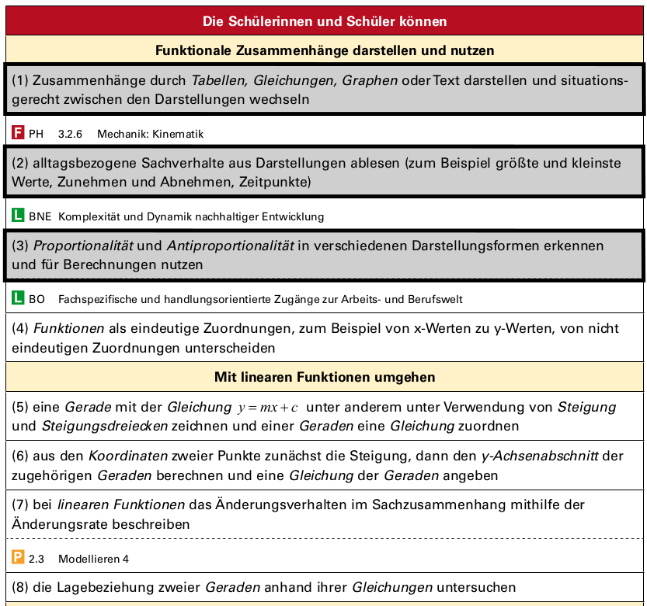
\includegraphics[width=0.7\textwidth]{img/bildungsplan2.png}
    \caption{Leitidee Funktionaler Zusammenhang für Klasse 7/8 aus dem Bildungsplan 2016.}
    \label{fig:bildungsplan} 
\end{figure}

\end{document}
